%%%%%%%%%%%%%%%%%%%%%%%%%%%%%%%%%%%%%%%%%%%%%%%%%%%%%%%%%%%%%%%%%%%%%%%%%%%%%%%%
%2345678901234567890123456789012345678901234567890123456789012345678901234567890
%        1         2         3         4         5         6         7         8


%\documentclass [UTF8]{ctexart}

%\documentclass[letterpaper, 12 pt, conference]{ieeeconf}  % Comment this line out
                                                          % if you need a4paper
\documentclass[a4paper, 12pt, conference]{ieeeconf}      % Use this line for a4
                                                          % paper
\usepackage{fontspec}
%\setmainfont{Microsoft YaHei}
%\setmainfont{SimSun}
\XeTeXlinebreaklocale "zh"
\XeTeXlinebreakskip = 0pt plus 1pt
%\IEEEoverridecommandlockouts                              % This command is only
                                                          % needed if you want to
                                                          % use the \thanks command
%\overrideIEEEmargins
% See the \addtolength command later in the file to balance the column lengths
% on the last page of the document

\usepackage{hyperref}
\usepackage{ctex}       %支持中文
\usepackage {subcaption}
\usepackage{graphicx}
\usepackage{stfloats}
%\usepackage{natbib}
%\usepackage{natbibspacing}


\hypersetup{
    colorlinks=true,
    linkcolor=blue,
    filecolor=magenta,      
    urlcolor=cyan,
}

% The following packages can be found on http:\\www.ctan.org
%\usepackage{graphics} % for pdf, bitmapped graphics files
%\usepackage{epsfig} % for postscript graphics files
%\usepackage{mathptmx} % assumes new font selection scheme installed
%\usepackage{times} % assumes new font selection scheme installed
%\usepackage{amsmath} % assumes amsmath package installed
%\usepackage{amssymb}  % assumes amsmath package installed

\title{\LARGE %\bf
\heiti
云计算安全研究综述
}

%\author{ \parbox{3 in}{\centering Narshion Ngao*
%         \thanks{*Use the $\backslash$thanks command to put information here}\\
%         Msc. Computer Systems - 2018\\
%         Jomo Kenyatta University of Agriculture \& Technology \\
%       
%}}

\author{2020-05-15 \\% <-this % stops a space
面向信息技术的沟通技巧
}


\begin{document}



\maketitle
\thispagestyle{empty}
\pagestyle{empty}


%%%%%%%%%%%%%%%%%%%%%%%%%%%%%%%%%%%%%%%%%%%%%%%%%%%%%%%%%%%%%%%%%%%%%%%%%%%%%%%%

\section{研究背景与意义}

\subsection{背景}
云计算(Cloud Computing)作为一种新型的宏观分布式计算技术,近年来得到了迅速的发展与普及,被视作当今最具发展潜力的领域之一。云计算通过动态分配海量的计算资源,具有高可用性、可动态扩展等特点,允许用户在云端共享数据与计算信息。但在云计算服务高速发展的同时,这项技术的安全性能也受到了广泛关注,在经历过一系列安全事故后,工业界和学术界迅速展开了一系列对其安全原理和防御策略的研究,研究领域诸如但不局限于数据隔离、访问管理、加密存储等技术。同时,云计算的安全性能,也在一定程度上决定了云计算发展的成功与否,将直接影响其可靠性以及用户的信任度。
\subsection{意义}
如今,云安全问题已经成为制约云服务发展的重要因素,各大云服务商的安全事故屡见不鲜,几乎无一幸免:2009年3月,Google大量用户的云数据遭到外泄;2012年4-12月当中,亚马逊的地区数据中心多次宕机;2014年9月,苹果iCloud发生严重信息泄露,上百位明星的账户图片被公之于众,影响恶劣;2018年3月,安德玛(UA)饮食健身应用上1.5亿账户数据被黑客窃取。由于互联网、金融、医疗、教育等众多重要领域与云计算服务联系紧密,一旦云计算服务产生中断,隐私信息遭到泄漏或丢失,这些领域的企业或个人都将遭到巨大的、无法挽回的损失。因此,研究并提高云计算服务的安全能力,将对云计算的发展和网络空间安全产生重要意义。

%\begin{enumerate}有序列表
%  \item Automatic Detection and Correction of Vulnerabilities using Machine Learning by Robin Tommy and others.
%\end{enumerate}


%%%%%%%%%%%%%%%%%%%%%%%%%%%%%%%%%%%%%%%%%%%%%%%%%%%%%%%%%%%%%%%%%%%%%%%%%%%%%%%%
\section{发展脉络}
%\subsection{Authors}子标题
%123
%\subsection{Authors}
早在上个世纪60年代,计算能力可以作为商品进行流通的理念就已出现,相应的安全理念也逐渐开始发展,从2006年开始,Amazon、IBM、Google等互联网企业相继推出了云服务,这也标志着云计算商业化开始普及,与此同时,云计算安全领域的研究开始成体系地发展起来。2009年,云安全联盟(CSA)成立,并开始发布《云计算安全指南》,标志着云计算安全领域发展的里程碑事件,推进了一系列行业标准的建立。

如今,云计算安全领域的基础建立在美国国家标准技术研究院(NIST)提出的安全云模型之上,它的组成含五个基本特征:应需自助服务、开放网络访问、资源池、快速延展性、监视服务,三个服务模型:软件即服务(SaaS)、平台即服务(PaaS)、基础架构即服务(Iaas),以及四个部署模型:私有云、社区云、公共云和混合云。在此之上,云安全的相关标准和技术还将继续推动行业进步。

%\begin{itemize}无序列表
%    \item Components of a Machine Learning IDS System
%    \item Implementation
%    \item Case Study
%\end{itemize}

\section{研究现状}
%\subsection{}
%\subsection{}
“A Review on Cloud Security”作为一篇综述性文章,主要从理论与模型,可能威胁和预防手段等角度阐述了云计算安全领域的重要研究方向。其中,作者将这些部分拆分为系统可用性、建模整合度、数据隐私,攻击分析等14个子模块,其中以攻击分析为重点阐述了当前云计算安全面临的主要威胁和常见攻击思路,作者在此指出:当攻击信号特征码可识别时,入侵防御系统(IPS)有效;当无法识别,且攻击者恶意占用处理器资源、网络带宽时,云服务可能会被迫关闭正常用户的使用需求,造成宕机;如果攻击者通过云服务器阵列尝试破解加密密钥时,就可能实现云对云的攻击,会造成巨大危害\cite{10.1145/2523514.2527013}。

如何有效防范攻击,作者在文中只提出了一条建议:使用者可以在端点实施主机防御入侵系统(HIPS)以阻止DoS发生。除此之外,文章其它部分并没有列举出其他安全策略,在解释潜在威胁后,缺乏对解决方案部分内容的整理,尤其是缺少针对某种不安全事件的具体处理措施或案例,这是我认为本篇综述的不足所在。

“Cloud Security Metrics”一文中详细讲解了国际电信联盟(ITU)提出的数据网络与开放通信安全体系(OSCA)的结构,即一种由三个结构层次组成的通信体系模型,分别是:基础结构层、服务层和应用程序层,分别用于提供电信功能的硬件和软件基础、计算可计费的客户流量、吸引用户为控制层服务付费。同时,作者指出,为避免这些层次中某一部分受损导致整个系统宕机,就必须保证局部安全问题在单层次内便能够修复。在此基础上,作者提出了支持基准威胁设置的层次结构,用以提高整个系统的安全性能\cite{bayuk2011cloud},具体实现如下图所示:

\begin{figure}[htbp]
\centering
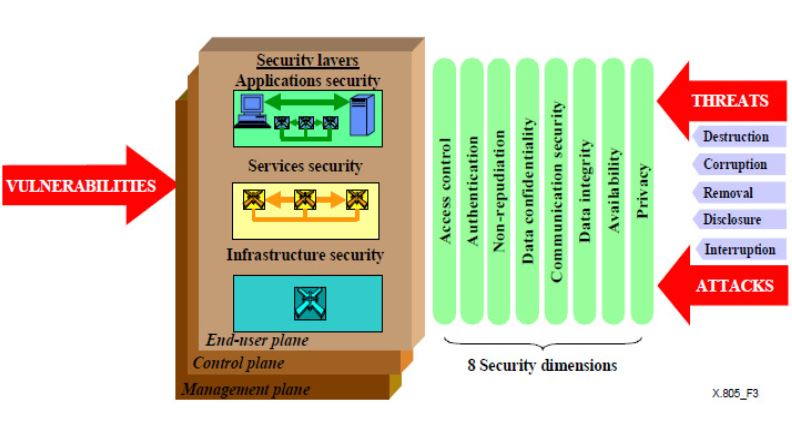
\includegraphics[width=3in]{pic/图1}
\caption{ITU安全模型}
\label{fig:1}
\end{figure}

由于这篇文章是基于通信模型体系结构进行的云安全模型研究,故内容存在较多通信领域的术语,并且由于学科交叉,专业紧密度可能不足,对于计算机专业的读者可能有些难以理解,更适合具有通信领域基础的学者研读。

云计算模型的多层架构决定了用户无法获得数据的完全控制权,与常规计算相比,这种控制力的降低可能会导致存在数据盗用风险。在“A Security Analysis of Amazon’s Elastic Compute Cloud Service”一文中,作者以亚马逊的动态云计算服务为例,将云上虚拟服务器与传统服务器机房进行对比研究。作者在EC2平台上进行的AMI安全性测试表明:当前云计算的资源池与弹性存储特性具有安全隐患,在存在资源存储的情况下,恶意用户可能会通过数据恢复技术,获取先前用户遗留的数据\cite{balduzzi2012security}。在后续的测试实验中,作者在此基础上,通过数据恢复非法获取了98\%的遗留机器映像文件,并证实了此前的漏洞猜想。在这篇文章中,作者在前期做了非常充分论证,并通过实验证实了自己的猜想,但是由于实验环境只选择了亚马逊EC2平台,而没有将猜想尝试运用于其他云计算系统,因此,在结论的普适性上,文章的内容有所不足。

与这篇文章研究内容相近的还有文献“Data Security and Privacy Protection Issues in Cloud Computing”,作者在文中分析了数据删除的软件可行性以及硬件存储介质的物理特性,指出:由于云计算服务器的多租户(Multi-Tenancy)性质,可能造成潜在的介质清理不当风险\cite{chen2012data}。即:当用户的数据被删除时,其备份在CSP端的物理存储仍然存在,这种情况下,其他用户的数据恢复操作,可能会触发系统的空间分配漏洞,导致无意中泄露敏感信息,进而对前一位用户的信息安全造成重大威胁。将本文与上一份论文对比,我认为,这篇文章在这个方向的论述与研究缺乏实验数据的支撑,导致说服力较弱,这也是本文的缺陷所在。

另一篇研究云计算安全体系的文献“Study on the Security Models and Strategies of Cloud Computing”提出了一种名为云管道模型(CCM)的结构,这种模型分别以内部与外部、私有与开放、内源与外源、周边与非周边作为不同的数据通道划分依据(见图2),对系统的安全性进行了模块化的描述,使用户能更直观地了解云计算当前安全控制措施的部署情况,从而更容易纠正自己可能的决策失误,实施更安全的操作\cite{che2011study}。由于这部分的研究篇幅较少,因此对一些其他特性的叙述,如:离岸与在岸,缺乏进一步展开,浅尝辄止,这也是本文美中不足的一点。

\begin{figure}[htbp]
	\centering
	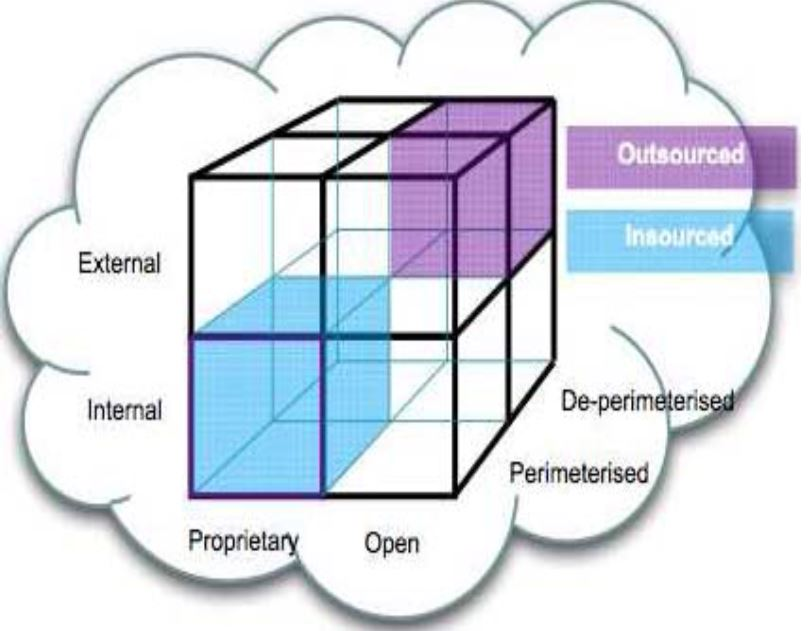
\includegraphics[width=3in]{pic/图2}
	\caption{云管道模型}
	\label{fig:2}
\end{figure}

“Cloud computing security: The scientific challenge, and a survey of solutions”研究了数据在存储时的一项加密技术——完全同态加密(FHE),其原理主要为明文数据的所有者与密文的持有者具有相通的权限设置。不同于普通加密的单向性,FHE允许密文持有者对密文执行某些操作,并将操作同态化到明文\cite{ryan2013cloud}。

以普通RSA算法为例:假设密文c1是在明文m1的公共密钥pk下的加密,而c2是在m2的相同密钥下的加密,即:$$c1 = enc(pk,m1)$$ $$c2 = enc(pk,m2)$$之后,将密文相乘得到的结果解密,则结果两个明文相乘后的结果相同。即:如果sk是与pk相对应的解密密钥,则有$$m1 \times m2 = dec(sk,c1 \times c2)$$本文章的论述有理有据,通过举例将思路呈现为数学公式,使读者容易理解。如果在普通RSA算法的基础上延展到其他加密算法或特殊的RSA,如其他文献中提到过的嵌入式RSA,会使文章更有层次感,结果更有说服力。



文献“An Analysis of the Cloud Computing Security Problem”还引入了安全工程活动中软件开发生命周期(SDLC)的概念,包括对安全需求的确定、潜在威胁的建模、系统模型的安全扩充以及相应的代码维护。在平台即服务(PaaS)的模式下,基于云的应用程序可以借助可重用的安全组件集合,并支持自适应安全性\cite{almorsy2016analysis}。作者还指出,这类自适应应用程序需要将软件的安全实施与管理权限移交给云安全性管理,云安全性服务和安全性控制,以满足对此类系统施加的新的云计算安全性需求。这一部分缺乏实例叙述,读者在阅读时容易陷入很多专有名词中,并且由于是借鉴了软件工程开发的理论,因此不太适合初学者学习。

\begin{figure*}[hb]
	\centering
	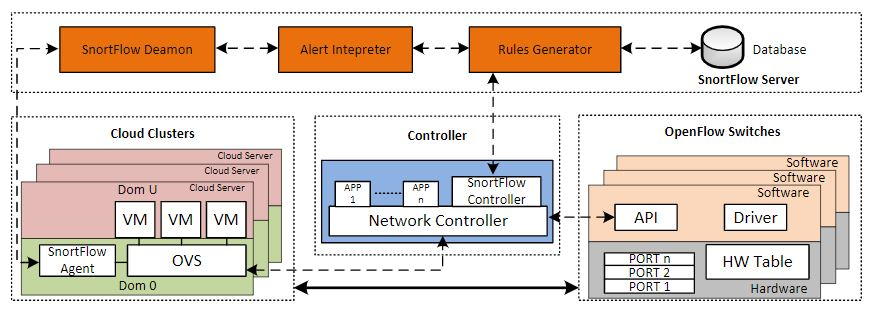
\includegraphics[width=6in]{pic/图3}
	\caption{SnortFlow系统架构}
	\label{fig:3}
\end{figure*}


为保障云计算中通信和网络的安全,研究者们提出了不同解决方案。“Snortflow: A OpenFlow-based Intrusion Prevention System in Cloud Environment”的作者设计了一款名为SnortFlow的系统,用于在云环境中进行入侵防御,SnortFlow系统的原型是在基于Xen的云上进行构建和测试的,同时借鉴了Snort和OpenFlow系统的功能\cite{xing2013snortflow}。在系统内部,由称为demon的程序组件收集系统的可疑流量,并发送警报到信号解释器中,经过转义后,传送至约束生成器并为可疑流量设置访问约束,同时将其转发到开放流设备,重新配置网络流量,以阻止可能出现的入侵。经过多次评估与实验,SnortFlow系统在流量分析和防止入侵方面均有良好的性能表现。本篇文章结构紧凑,图文并茂,在理论阐释之外提供了充分的横向对比实验数据,有力地论证了自己的结论。



基于CSA的访问控制和身份管理理念,文献“Design Role-Based Multi-Tenancy Access Control Scheme for Cloud Services”提出了基于角色的多租户访问控制(RB-MTAC)方案,要求用户向云进行注册,并获得Unique-ID作为身份凭证。在进入云计算系统时,用户必须通过平台中身份管理模块的认证:根据注册用户的身份凭证和信息表,识别并定向连接到RB-MTAC数据库的角色分配模块,并为不同的用户分配不同的功能角色,赋予各自的处理特权。这种解决方案能够实现应用层的独立和数据隔离,从而提高云多租户服务的处理性能,增强了云计算平台的安全性和隐私性\cite{yang2013design}。本文作者提出的理念是对当前多租户服务框架的改进版,并且提供了实验数据支撑,由于大多数入侵事件都是由于原本的访问控制结构存在漏洞,造成恶意身份盗取用户数据,而这项研究的出现将在一定程度上改变这一现状,本文的不足之处在于中间部分的源代码占用篇幅过多,占据全文1/7的空间,若改成更精简的伪代码将提高读者的阅读体验。

根据CSA提出的另一条有关数据安全性和密钥管理的建议,文献“Security and privacy for storage and computation in cloud computing”的作者提出了一种安全存储协议SecCloud,目的在于不仅可以保护用户上传到云中的数据,还可以保护对这些数据执行的计算操作。作者提出,SecCloud采用双线性配对的方案(循环的加法乘法组合)为用户,云和受信任的第三方生成密钥。用户从CSP获取动态存储空间后,协议首先将数据分为m个子消息,之后发由受信任的第三方验证者签名,再经由会话密钥加密,最后将数据和签名一起发送到云。其中,会话密钥由用户和云通过双线性Deffie-Hellman计算得出,接收到云后,云将解密数据,验证签名并将其存储在云中的指定分区,从而确保了计算安全性。除数据上传外,SecCloud还可以通过重建Merkle树的方法,验证数据是否存储在云的正确分区上,为了减少计算冗余,验证程序采用概率抽样代替整个树的构建\cite{wei2014security}。为验证可行性,作者还构建了SecHDFS——作为SecCloud测试用的云计算实验平台,并实验证明SecCloud上传文件的抗干扰能力强于原始协议,论证了自己的理论。与前一篇文献的出发点相似,作者同样是基于CSA提出的安全性建议,在已有协议框架的基础上进行了整合与改进,具有较大的实用价值,同时理论论证完善,实验设计合理,兼顾设计与实现,十分适合作为入门文献学习。


\begin{figure}[htbp]
	\centering
	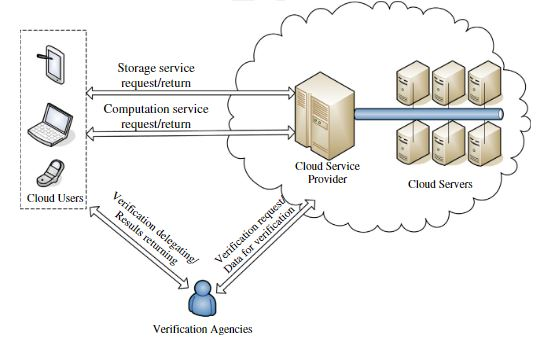
\includegraphics[width=3in]{pic/图4}
	\caption{SecCloud云计算架构}
	\label{fig:4}
\end{figure}

如今,在云安全领域,学术界研究重点主要是围绕系统化模型的架构以及针对当前云端解决方案可能存在的漏洞进行改进,同时,对云安全策略的探索逐渐呈现出多领域融合的研究趋势,如\cite{bayuk2011cloud},这也说明,在如今学科交叉的大背景下,学术界对云计算安全的理论研究正在走向复合化,多元化,而这将更好地推动云计算服务的多领域发展,并为以后的应用需求普及起到积极促进作用。

\section{未来前景}

云计算安全作为一项新兴技术,经过了十几年来的高速发展,如今已经成为了工业界以及学术界研究的热门领域,具有起步晚,发展快的特点,目前总体上仍处于探索与拓展阶段。

根据对前一部分文献阅读中了解到的潜在研究领域以及对现有保护方案缺陷的总结,结合近年来云计算服务发展趋势,笔者得出了以下思考:

\subsection{进一步研究课题}

\subsubsection{自适应安全策略}
\ 

当前的安全威胁与云计算环境时刻处于动态变化之中,面临着不断进化的攻击方式,以往适用于很多操作系统的静态安全机制,将难以胜任云系统的防卫工作。而相对的,自适应安全机制则能够对用户的交互记录和当前环境进行动态信任评估,并以此向用户提出的操作建议,对于可能进行的恶意行为则限制其权限,以达到动态限制的目的。

目前学术界对基于自适应配置的安全模型研究已有了初步进展,如:基于信任的自适应交互框架,但当前的研究距离实际的安全对策、漏洞处理、配置映射和实验环境搭建仍有相当的距离,但可以预见的是,自适应安全策略将是云系统与用户交互层重要的风险屏蔽手段,同时也是云消费者对安全环境建立信任感的关键所在。


\subsubsection{云虚拟化安全}
\ 

目前,针对云端虚拟化的攻击手段主要有两种:
\begin{enumerate}
	\item  回滚攻击 
	\subitem
	黑客通过劫持云端虚拟机,执行旧版本的管理程序,从而撤销最新的安全更新并暴露程序漏洞,实现入侵系统。
	
	\item 虚拟机逃逸攻击 
	\subitem 黑客启用访客级别的虚拟机(VM)并攻击其管理程序,并从VM管理程序的控制下逃逸,进而接管管理程序并获得对本地OS文件的访问权限,达到入侵本地存储的目的,并入侵管理程序控制下的其他VM设备。

\end{enumerate}


这两种情况往往出现在系统管理程序与VM之间的隔离较弱或没有隔离时,当前的云服务对此供给的防御策略仍具有一定局限性,如异常检测技术对隐通道的检测效率低,且检测过程存在泄漏隐私的风险等。而近年来,学术界也已经开始了在此的领域研究,并已经提出了通过建立三层虚拟网络框架来对VM通信进行加密与隔离的概念。在未来一段时间内,相关领域的模型构建和安全策略还将得到进一步的发展。

\subsection{发展方向展望}
\subsubsection{结合硬件支持的云模式}
\ 

单纯依赖软件的安全策略可能难以防范从云端对本地OS的攻击,同时由于云服务质量受到当前网络状况、云平台流量、私人访问控制影响,难以提供长期稳定的服务。另一方面,移动硬盘的存储能力较云端弱,且大多不具备计算能力,但服务能力稳定,信息存放安全。因此,我们可以考虑将两者结合的方式,通过用户端的硬件产品增强云服务表现,并在更稳定的环境中为数据提供额外保护,让用户体验到像在专用设备中一样安全的云计算服务。

\subsubsection{与深度学习技术融合保护}
\ 

如今,深度学习技术已经被广泛的应用于网络空间安全、物联网安全、线下监控体系等安全领域之中,并取得了出色的效果。由于云服务同样是一种多用户分布式参与的体系,因此可以将深度学习技术融入到云计算安全策略当中,通过云服务的海量数据优势,跟踪并研究用户安全行为模式,并自动为不同的用户提供其可能采纳的安全性配置建议,从而使云安全更加客制化,提高消费者的云安全意识与使用体验。

\subsubsection{通过5G技术建立云安全信息网}
\ 

随着5G技术的迅速推广,其强大的信息处理传输能力,使得海量数据能够得以整合,并建立相互联系。可以通过5G技术的连接作用,建立云服务用户之间的信息联系图,在发现平台可能存在的系统漏洞时,自动向行为模式相近的用户提供针对性保障,同时,如果有用户通过云端窃取其他受控用户的信息,则可以及时切断其与其他用户的信息通道,降低受损数据规模,保障用户的信息安全。


\section{见解与感想}

在过去的十余年间,云计算服务深刻地改变了我们对数据的理解:从过去手动将数据复制到移动硬盘,到如今iCloud实现自动备份;从过去合租服务器,到今天云计算触手可得,云服务的模式走进了一个又一个领域,基于云的商业机会也如雨后春笋般破土而出。但是,云安全的威胁规模也在迅速扩张,其潜在危害随用户数量的增长正不断放大,云计算的安全性,正变得前所未有的重要。

云服务在计算方面的优势,在安全领域转眼间又变成了劣势,虚拟化、多租户、资源池共享等特征使得用户同样的行为,熵值变得更高,系统混乱程度增加,加之云资源价值高,组织者宏观控制能力缺乏,这些都使得云计算容易成为黑客攻击的对象。正如之前所提到的,学术界近十年来在云计算领域仍处于不断拓展阶段,而目前使用的安全策略仍然是针对现有攻击方式进行的有限保护,对于可能出现的新型安全问题则缺乏前瞻性研究,在进度上略有滞后。但同时我们也应该看见,作为新兴领域,云计算的安全问题在近年来得到了迅猛发展,安全事故率也呈现出逐年稳中向好的态势,这都离不开工业界和学术界长期的努力。

就像长矛与盾牌的共同进化一样,云计算安全与威胁也将保持长期共存、相互促进的关系,世界上没有绝对安全的系统,也没有战无不胜的黑客技术,唯有时刻保持警惕,在失败中不断汲取教训,云计算安全性的发展进步,才能生生不息。


%添加宏包:
%\usepackage{natbib}
%\usepackage{natbibspacing}
%设置参考文献间的间距
%\setlength{\bibspacing}{0\baselineskip}


%设置文献的样式
\bibliographystyle{plain} 
%添加自己的bib文件
\bibliography{Reference}

%\bibitem{c2} Sanjay Kumar, Ari Viinikaineny and Timo Hamalainenz, 2016. Machine Learning Classification Model For Network Based Intrusion Detection System
%\bibitem{c3} Gauri Kalnoor and Jayashree Agarkhed, 2016. Preventing Attacks and Detecting Intruder for Secured Wireless Sensor Networks.
%\bibitem{c4} Hsiu-Chuan Huang, Zhi-Kai Zhang, Hao-Wen Cheng, and Shiuhpyng Winston Shieh, 2017. Web Application Security: Threats, Countermeasures, and Pitfalls







\end{document}
